\documentclass{scrartcl}
% Comment the following line to NOT allow the usage of umlauts
\usepackage[utf8]{inputenc}
\usepackage[spanish]{babel}
\selectlanguage{spanish}
\usepackage{xcolor}
\usepackage{tcolorbox} %para cajas de texto
\usepackage{sectsty}
\usepackage{hyperref}
%\usepackage{color}
\usepackage{bbding}
\definecolor{hd}{rgb}{0.2,0.2,0.7}
\definecolor{tit}{rgb}{0.1,0.4,0.7}

% Fifure in italics

\usepackage[format=plain,
labelfont=it]{caption}

\sectionfont{\color{hd}} 
\subsectionfont{\color{hd}} 
\subsubsectionfont{\color{hd}} 

% save figure on top
\makeatletter
\setlength{\@fptop}{0pt}
\makeatother

\graphicspath{{../figs/}}

% Uncomment the following line to allow the usage of graphics (.png, .jpg)
%\usepackage{graphicx}
\title{\color{tit} Doing bayesian data analysis\\
		by Kruschke}
	\subtitle{Revisión} 
\author{\normalsize J. E. Alcalá \\
		\normalsize CEIC, Universidad de Guadalajara} 
\date{\today} 
% Start the document
\begin{document}
\maketitle 
	\section{Capítulo 2}
	
	\textsf{\textbf{Ideas fundacionales:}}
	
	\begin{enumerate}

		\item Reasignación de credibilidad a través de las posibilidades.
		\item Las posibilidades se representan como parámetros de modelos matemáticos.
	
	\end{enumerate}
	
	\subsection{Reasignación a través de posibilidades}
		\begin{tcolorbox}
		\textsf{\textbf{Ejemplo 1:}}		
		
			\textbf{A.} Observación: camino mojado. \\
			\textbf{B.} Posibilidades-creencias: \{llovió, borracho tiró su bebida, etc.\}. \\
			\textbf{C.} Nuevas observaciones: \{humedad se extiende a lo lejos, humedad está localizada\}. \\
			\textbf{D.} Reasignación: la ocurrencia de un elemento del conjunto en \textbf{C} modifica la credibilidad en alguno de los elementos de \textbf{B} para los cuales el elemento en \textbf{C} podría haberlo causado. 
		\end{tcolorbox}
		
		En el \textsf{\textbf{Ejemplo 1}}, observar que la humedad se extiende a lo lejos podría reducir las posibilidades de ``borracho tiró su bebida'', por otro lado, observar que la humedad está localizada reduce las posibilidades de ``llovió''. 
		
		Las creencias depositadas en los elementos de \textbf{A} son \textit{a priori} en el sentido de que, en el momento en el que se enuncian (junto con un valor numérico entre 0 y 1 de acuerdo al \textit{grado} en el que se crea en ellas; la suma de la credibilidad debe dar 1), no se ha recolectado evidencia de su ocurrencia. 
		
		Las nuevas obervaciones son datos. La reasignación de credibilidad es \textit{a posteriori} porque sucede después de haber recolectado datos. Dado que estos datos redistribuyen los valores numéricos (entre 0 y 1), una vez recolectamos datos no creemos en todas las posibilidades al mismo grado que antes de la recolección.
		
		La credibilidad posterior puede servir como credibilidad \textit{a priori}, es decir, el conjunto \textbf{D} $\rightarrow$ \textbf{B'}, y el proceso se repite, lo que se conoce como \textit{actualización bayesiana}. 
		
		\subsubsection{Datos ruidosos: inferencia probabilística}
		
		Los datos tienen relaciones \textit{probabilísticas} con las causas subyacientes. 
		
		\begin{tcolorbox}
			Datos \textit{ruidosos}
			\tcblower
			1. Los datos son producto de mediciones imperfectas. \\
			2. Cada dato resultado de una medición imperfecta es diferente a otros datos. E.g., $x_1 \neq x_2 \neq x_3$.\\
			3. Además de las mediciones imperfectas, los datos en sí pudieron ser generados por un proceso no determinístico. \\
			4. Esta variabilidad acota la exactitud con la que inferimos \textit{qué} pudo haber generado esos datos (i.e., cuál es la causa subyaciente).\\
			\textsf{\textbf{Ejemplo 2:}}\\
			La tasa de respuesta en un programa IV 30 s varía de animal en animal, sesión a sesión en el mismo animal y bajo diferentes condiciones, como grado de privación o tipo de reforzador utilizado. \\
			Además, el operando puede descalibrarse, no detectar respuestas muy contiguas, o respuestas dadas con poca fuerza, etc. \\
			\textsf{\textbf{Nota:}}\\
			\HandRight \hspace*{0.1em} Se asume que existe un proceso `verdadero' que da lugar a la variable observada. Por ejemplo, que la tasa es $\mathcal{R}$, pero obtenemos $\hat R$, un estimador de la \textit{tasa verdadera}, o la tasa que se tendría si no hubiera errores de medición. $\mathcal{R}$ podría ser una variable aleatoria, pero los errores de medición añaden \textbf{incertidumbre} a la \textit{forma} que esa variable toma. 
		\end{tcolorbox}
	
	\textbf{\textsf{Resumen:}}
	\begin{enumerate}
		\item La esencia de la inferencia bayesiana es la reasignación de la credibilidad.
		\item La credibilidad inicial (\textit{a priori}) refleja el conocimiento previo sobre las posibilidades, y puede ser muy vago (en cuyo caso no se beneficia a alguna posibilidad por encima del resto).
		\item Las posibilidades inconsistentes con los datos pierden credibilidad.
	\end{enumerate}

	\subsection{Las posibilidades son parámetros de modelos}
	
	Dado que las mediciones producen datos variables, la mejor forma de representar las creencias del proceso generador de datos es con probabilidad. 
	
	Distintas distribuciones (o densidades) de probabilidad implica que se debe elegir cuál de ellas (qué modelo) representa mejor las creencias. Luego de elegir el modelo probabilístico (e.g., distribución normal, binomial, etc), se debe elegir qué \textit{qué parámetros} determinan la distribución (e.g., en distribución normal son $\mu$ y $\sigma$). 
	\begin{itemize}
		\item ¿Cuánta confianza tenemos en las posibilidades sobre las que depositamos nuestras creencias? Si no es mucha, nuestras creencias son \textit{vagas}.
		\item Si las creencias son vagas, debemos escoger un modelo \textit{a priori} acorde, por ejemplo, uno donde todas las posibilidades tengan la misma probabilidad de ser verdad (e.g., distribución uniforme, o distribución normal con una desviación estándar muy (muy) grande; ver la Figura ~\ref{fig:fig1}).
	\end{itemize}
		
	\begin{figure}[t!]
		\centering
		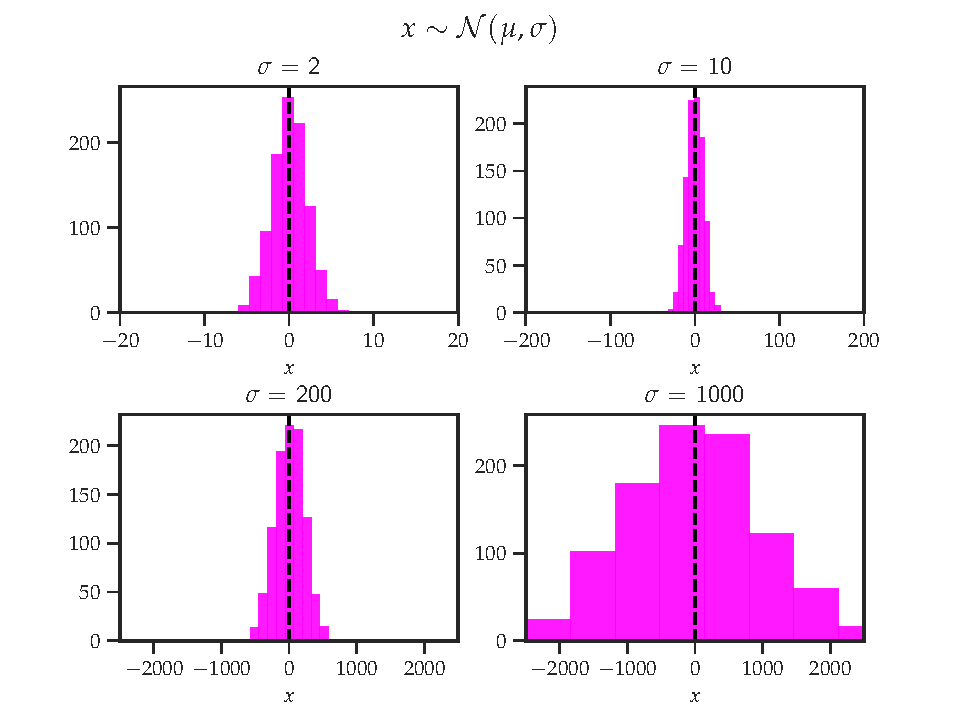
\includegraphics[width=\textwidth]{Figure_1.pdf}
		\caption{Distribuciones normales con mismo $\mu$ pero distinto $\sigma$, que refleja diferentes grados de `vaguedad'. Conforme $\sigma \rightarrow \infty$, las posibilidades son equiprobables. Notar que los ejes en $x$ cambian de límites. En el panel inferior derecho, si restrinjimos los valores de $x \in [-100,100]$ la distribución se vería casi plana.}
		\label{fig:fig1}
	\end{figure}
	
	\subsection{Pasos de la inferencia bayesiana}
	
	\begin{tcolorbox}[colback=red!5!white,colframe=red!75!black]
		\begin{enumerate}
			\item Identificar qué datos (o variables) responden a una pregunta. 
			\item Definir modelo descriptivo para los datos, con la forma matemática adecuada.
			\item Especificar la distribución \textit{a priori} de los parámetros. 
			\item Usar inferencia bayesiana para reasignar credibilidad a los parámetros. 
			\begin{itemize}
				\item Interpretar la distribución posterior con respecto a las la teoría.
			\end{itemize}
			\item Revisar que las predicciones posteriores se asemejen a los datos con precisión razonable (\textit{posterior predictive check}). Si no, volver al paso 2.
		\end{enumerate}
	\end{tcolorbox}
	
\end{document}
